\documentclass{lecturefig}
\usetikzlibrary{chains}
\begin{document}
\begin{frame}[fragile]
  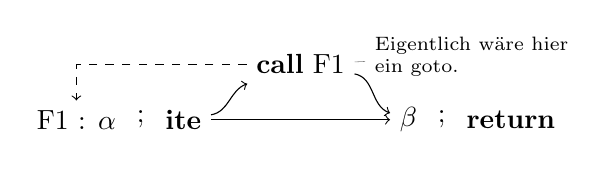
\begin{tikzpicture}[
    operation/.append style={rectangle, on chain},
    start chain,
    node distance=1mm,
    ]
    \def\seq{\node[on chain,inner sep=1pt] {;};}

    \node[operation] (entry) {F1 : $\alpha$}; \seq
    \node[operation] (ite) {\textbf{ite}};

    \node[operation, shift={(1em, 2em)},pin={[align=left,anchor=north west,font=\scriptsize]30:Eigentlich wäre hier\\ ein goto.}] (call) {\textbf{call} F1};

    \node[operation,, shift={(1em, -2em)}] (return) {$\beta$};\seq
    \node[operation] {\textbf{return}};


    \draw[->] (ite) to[out=10,in=200] (call);
    \draw[->] (call) to[out=-10,in=160] (return);
    \draw[->] (ite) to[out=0,in=180] (return);
    \draw[->,dashed] (call) -| (entry);
  \end{tikzpicture}
\end{frame}

\begin{frame}[fragile]
  \begin{tikzpicture}[every op/.style={fill=operatorcolor}]
    \begin{opAxis}
      \opString{$\alpha_1$, $\alpha_2$}
      \only<1>{\opString[minimum width=2em]{$\alpha_3$, $\beta_3$}}
      \only<2>{\opString[minimum width=4em]{\textbf{call} F1}}
      \opString{$\beta_2$, $\beta_1$}
    \end{opAxis}
  \end{tikzpicture}
  \end{frame}
\end{document}
